%-----------------------------------
% Kapitel 2: Theoretische und technologische Grundlagen
%-----------------------------------
\section{Theoretische und technologische Grundlagen}

Die Wissensbasis der Arbeit setzt sich aus drei Str\"angen zusammen. Abschnitt~\ref{itsm} kl\"art die Begriffe des IT-Service-Managements und beschreibt das Incident Management als denjenigen Handlungsrahmen, in dem der First-Level-Support t\"atig ist. Abschnitt~\ref{kiGrundlagen} behandelt K\"unstliche Intelligenz im Unternehmenskontext, grenzt regelbasierte Chatbots von Large Language Models ab und referiert den Stand der Forschung zum KI-Einsatz im IT-Support. Abschnitt~\ref{bpmnGrundlagen} f\"uhrt in die Prozessmodellierung mit BPMN~2.0 ein. Die Soll-Konzeption in Kapitel~4 verbindet diese drei Str\"ange, da sie eine fachliche Vorstellung des zu gestaltenden Prozesses, eine technische Vorstellung der Leistungsf\"ahigkeit und der Grenzen sprachverarbeitender Modelle sowie eine formale Sprache zur Darstellung des Ergebnisses gleichzeitig voraussetzt.

\subsection{IT-Service-Management und Incident Management}
\label{itsm}

Der First-Level-Support ist keine isolierte organisatorische Einheit, sondern Teil eines Rahmenwerks, das Aufgaben, Rollen und Abl\"aufe der IT-Leistungserbringung ordnet. Abschnitt~\ref{itilEinordnung} ordnet ihn deshalb zun\"achst in das ITIL-Framework ein und kl\"art die zugeh\"orige Begrifflichkeit. Abschnitt~\ref{incidentProzess} betrachtet anschlie{\ss}end den Incident-Management-Prozess mit seinem Ablauf und den daran beteiligten Rollen.

\subsubsection{Einordnung des First-Level-Supports im ITIL-Framework}
\label{itilEinordnung}

Das IT-Service-Management (ITSM) begreift IT-Leistungen nicht als Summe technischer Komponenten, sondern als Dienstleistungen mit einem definierten Nutzen f\"ur den Anwender. Kopperger, Kunsmann und Weisbecker beschreiben das IT-Servicemanagement als Instrument zur Planung, Steuerung und Kontrolle der IT-Services, dessen Aufgabe darin bestehe, deren Qualit\"at und Quantit\"at zielgerichtet, gesch\"aftsprozessorientiert, benutzerfreundlich und kostenoptimiert zu \"uberwachen und zu steuern\footcite[Vgl.][hier S.~422]{Tiemeyer2020}.

Als Referenzrahmen des ITSM hat sich die ITIL zu einem De-facto-Standard entwickelt, der ein einheitliches Referenzmodell bereith\"alt\footcite[Vgl.][S.~423]{Tiemeyer2020}. Marrone und Kolbe stellen in einer Befragung von IT-F\"uhrungskr\"aften fest, dass mit steigendem Umsetzungsgrad von ITIL die Zahl der wahrgenommenen Nutzeneffekte zunehme\footcite[Vgl.][hier S.~363]{MarroneKolbe2011}. Die Version ITIL~4 ersetzt die fr\"uhere, stark prozessorientierte Darstellung durch das Service Value System, in dem Practices an die Stelle einzelner Prozesse treten; eine Practice umfasst neben dem Ablauf auch Rollen, Werkzeuge und Wissen\footcite[Vgl.][Abschn.~5.1. Die ITIL~4 Foundation wird im Folgenden nach Abschnitten statt nach Seiten zitiert, da die Abschnittsnummerierung ausgabenunabh\"angig ist.]{AXELOS2019}. Die vorliegende Arbeit untersucht von der Practice Incident Management allein den Bearbeitungsablauf und verwendet daf\"ur weiterhin den Begriff Prozess, da die Modellierung in BPMN auf diese Ablaufebene zielt.\footcite[Vgl.][S.~447]{Tiemeyer2020}

Innerhalb dieses Rahmens nimmt der Service Desk als Practice die Vermittlungsfunktion zwischen Nutzern und IT-Organisation wahr\footcite[Vgl.][Abschn.~5.2.14]{AXELOS2019}. Er bildet den zentralen Anlauf- und Kontaktpunkt f\"ur alle Anfragen, nimmt die Kontakte \"uber unterschiedliche Kan\"ale auf, strukturiert sie und f\"uhrt sie der Weiterbearbeitung zu; zu seinen Aufgaben z\"ahlen das Registrieren und Nachverfolgen von St\"orungsmeldungen sowie deren erste Pr\"ufung\footcite[Vgl.][S.~450]{Tiemeyer2020}. Hinzu kommt eine kommunikative Aufgabe, da der Service Desk die Wahrnehmung der IT-Organisation durch die Anwender pr\"agt.

Organisatorisch ist der Service Desk regelm\"a{\ss}ig in ein mehrstufiges Support-Modell eingebettet. Die IT-Serviceorganisation umfasst dabei ein dreistufiges Support-Konzept aus First, Second und Third Level mit einem gemeinsamen Single Point of Contact; der First-Level-Support bildet dessen erste Bearbeitungsinstanz, w\"ahrend die nachgelagerten Stufen \"uber Tiefenwissen zu einzelnen Systemen verf\"ugen\footcite[Vgl.][S.~476]{Tiemeyer2020}. Angestrebt wird die fallabschlie{\ss}ende Bearbeitung beim Erstkontakt, sodass eine Weitergabe nur dann erfolgt, wenn die L\"osung Spezialwissen oder erweiterte Berechtigungen erfordert. \autoref{fig:supportmodell} zeigt den Aufbau dieses Modells.

\begin{figure}[htbp]
	\centering
	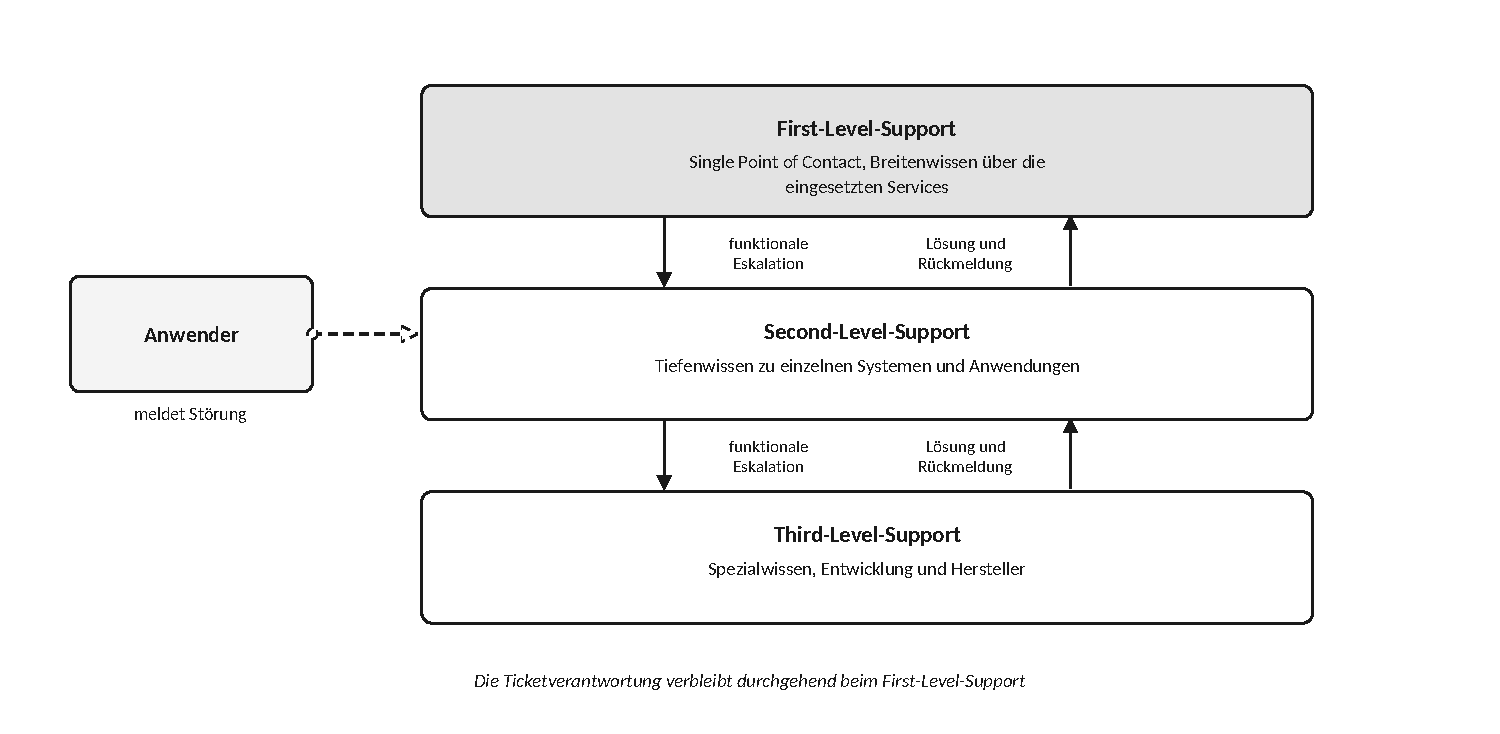
\includegraphics[width=\textwidth]{abb/abb2-support-modell.pdf}
	\caption{Mehrstufiges Support-Modell im ITSM}
	\label{fig:supportmodell}
	\par\vspace{0.4em}{\footnotesize Quelle: In Anlehnung an Kopperger/Kunsmann/Weisbecker (2020), S.~450 und S.~476.}
\end{figure}

Die eingehenden Anliegen sind begrifflich zu trennen. Ein Incident ist nach ITIL ein Ereignis, das den standardm\"a{\ss}igen Betrieb der IT-Services unterbricht; darunter fallen neben St\"orungen der Hard- und Software auch benutzerbezogene Ereignisse wie ein vergessenes Kennwort\footcite[Vgl.][S.~448]{Tiemeyer2020}. Ein Service Request betrifft demgegen\"uber ein regul\"ares, im Vorfeld vereinbartes Anliegen wie die Beantragung einer Berechtigung, ohne dass eine St\"orung vorliegt. Dem Problem Management f\"allt demgegen\"uber die Identifikation, Klassifikation und Behebung wiederkehrend auftretender Vorf\"alle zu, nicht dem First-Level-Support\footcite[Vgl.][S.~436]{Tiemeyer2020}. Wie die Bearbeitung eines Incidents im Einzelnen verl\"auft und welche Rollen daran mitwirken, betrachtet der folgende Abschnitt.

\subsubsection{Der Incident-Management-Prozess: Ablauf und Beteiligte}
\label{incidentProzess}


Das Incident Management verfolgt nach ITIL~4 das Ziel, den normalen Servicebetrieb nach einer St\"orung schnellstm\"oglich wiederherzustellen und die negativen Auswirkungen auf das Gesch\"aft gering zu halten\footcites[Vgl.][Abschn.~5.2.5]{AXELOS2019}[][S.~448]{Tiemeyer2020}. Von der regul\"aren Bearbeitung grenzt ITIL~4 den Major Incident ab, also eine St\"orung mit besonders hoher Auswirkung, f\"ur die eine eigene Verfahrensweise mit gesondertem Team und eigener Eskalationsstruktur vorgesehen ist\footcite[Vgl.][Abschn.~5.2.5]{AXELOS2019}. Die vorliegende Arbeit klammert diesen Sonderweg aus und betrachtet allein die regul\"are Bearbeitung. Vorrang hat somit die Wiederherstellung der Nutzbarkeit, nicht die abschlie{\ss}ende Ursachenkl\"arung. Die eingehenden Meldungen werden dazu priorisiert und kategorisiert, sodass die Bearbeitung nach ihrer Auswirkung differenziert erfolgt.\footcite[Vgl.][S.~448]{Tiemeyer2020}

Der Ablauf folgt dem Lebenszyklus eines Tickets. Die folgende Darstellung bleibt auf der Ebene, auf der das Referenzmodell selbst argumentiert, und benennt die Phasen und ihre Reihenfolge. Welche T\"atigkeiten in ihnen anfallen, wer sie ausf\"uhrt und welche Informationen dabei entstehen, untersucht Abschnitt~\ref{istProzess} mit Blick auf die Modellierung. Am Anfang steht die Erfassung und Protokollierung der Meldung, bei der der Service-Desk-Agent den Melder, den betroffenen Service, die Symptombeschreibung und den Zeitpunkt dokumentiert; unvollst\"andige Angaben erfordern R\"uckfragen, bevor die Bearbeitung fortschreiten kann\footcite[Vgl.][S.~448]{Tiemeyer2020}. Es folgt die Kategorisierung, die das Ticket einem Service, einer St\"orungsklasse und damit einer zust\"andigen Einheit zuordnet. Die Priorisierung leitet sich nicht aus der Kategorie ab, sondern aus dem Zusammenspiel von Auswirkung und Dringlichkeit. Die Auswirkung (Impact) erfasst, wie viele Anwender oder welche Gesch\"aftsprozesse betroffen sind, w\"ahrend die Dringlichkeit (Urgency) beschreibt, wie schnell eine Behebung erforderlich ist, bevor Schaden entsteht. Aus beiden Gr\"o{\ss}en ergibt sich die Priorit\"at des Tickets, an die Service Level Agreements (SLA) Zielzeiten f\"ur Reaktion und L\"osung binden.\footcite[Vgl.][S.~425]{Tiemeyer2020}

Auf dieser Grundlage beginnt die Erstdiagnose, in der der First-Level-Support die geschilderten Symptome mit dokumentierten L\"osungen abgleicht und die St\"orung, soweit m\"oglich, unmittelbar behebt. Bleibt dies erfolglos, geht das Ticket an eine nachgelagerte Einheit, die Untersuchung und Diagnose vertieft. Nach gefundener L\"osung wird der Servicebetrieb wiederhergestellt und das Vorgehen dokumentiert. Den Abschluss bildet die Dokumentation der St\"orungsl\"osung in der St\"orungsdatenbank, mit der der Prozess endet und die zugleich die Grundlage f\"ur die Bearbeitung vergleichbarer F\"alle bildet\footcite[Vgl.][S.~448]{Tiemeyer2020}. \autoref{fig:incidentablauf} stellt den beschriebenen Ablauf im Zusammenhang dar.

\begin{figure}[htbp]
	\centering
	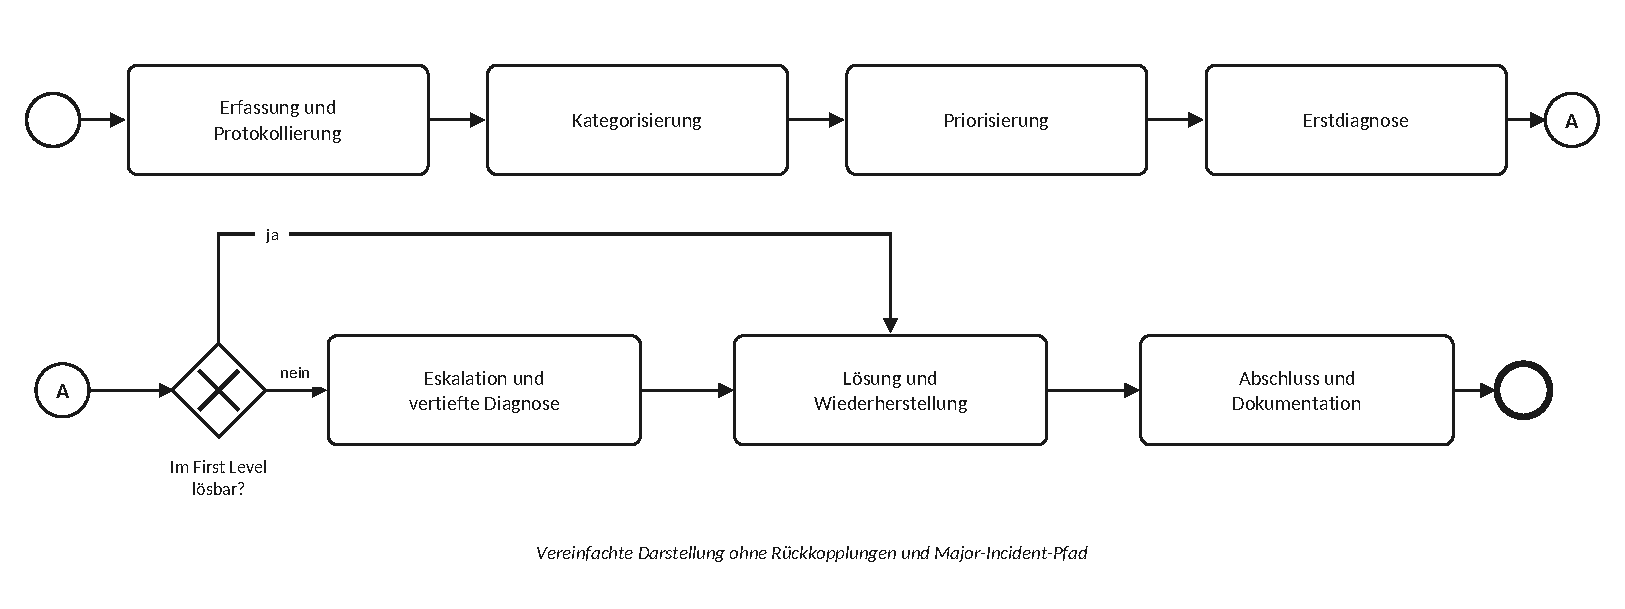
\includegraphics[width=\textwidth]{abb/abb3-incident-prozess.pdf}
	\caption{Ablauf des Incident-Management-Prozesses nach ITIL~4}
	\label{fig:incidentablauf}
	\par\vspace{0.4em}{\footnotesize Quelle: In Anlehnung an Kopperger/Kunsmann/Weisbecker (2020), S.~448.}
\end{figure}

Am Prozess wirken mehrere Rollen mit. Der Anwender meldet die St\"orung und beschreibt sie aus seiner Wahrnehmung, ohne technische Zuordnung. Der Service-Desk-Agent des First Levels nimmt die Meldung auf, klassifiziert sie und \"ubernimmt die Erstbearbeitung. Nachgelagerte Fachteams des Second- und Third-Level-Supports bearbeiten F\"alle, die Spezialwissen oder erweiterte Berechtigungen erfordern, w\"ahrend bei ausbleibender Behebung eine weitere Eskalation bis hin zu Entwicklern im eigenen Haus oder zum Service des Herstellers erfolgt\footcite[Vgl.][S.~448]{Tiemeyer2020}.

Als Hilfsmittel dient eine Fehlerl\"osungsdatenbank, in der bekannte Fehler samt zugeh\"origen Workarounds hinterlegt sind\footcite[Vgl.][S.~449]{Tiemeyer2020}. Der Prozess ist damit in weiten Teilen text- und kommunikationsbasiert, da Ticketbeschreibungen, R\"uckfragen und Wissensartikel in nat\"urlicher Sprache vorliegen. Sprachverarbeitende Verfahren treffen hier auf ein naheliegendes Anwendungsfeld, dessen technische Grundlagen Abschnitt~\ref{kiGrundlagen} legt.

\subsection{K\"unstliche Intelligenz im Unternehmenskontext}
\label{kiGrundlagen}

Der Begriff Chatbot umfasst Systeme h\"ochst unterschiedlicher Leistungsf\"ahigkeit. Abschnitt~\ref{chatbotAbgrenzung} grenzt deshalb regelbasierte von generativen Ans\"atzen ab, Abschnitt~\ref{llmFunktion} erl\"autert die Funktionsweise und die F\"ahigkeiten von Large Language Models, und Abschnitt~\ref{aiopsStand} arbeitet den Stand der Forschung zum KI-Einsatz im IT-Support und im Bereich Artificial Intelligence for IT Operations (AIOps) auf.

\subsubsection{Abgrenzung von regelbasierten Chatbots zu Large Language Models (LLMs)}
\label{chatbotAbgrenzung}

Chatbots sind dialogbasierte Systeme, die Eingaben in nat\"urlicher Sprache entgegennehmen und beantworten. Der regelbasierte Ansatz geht auf ELIZA zur\"uck, das in den 1960er-Jahren Konversation durch schlichten Musterabgleich nachahmte\footcite[Vgl.][hier S.~2]{Adamopoulou2020a}. Adamopoulou und Moussiades unterscheiden Chatbots nach der Art der Antworterzeugung. Regelbasierte Systeme bestimmen ihre Antwort \"uber Musterabgleich, Entscheidungsb\"aume und hinterlegte Skripte, weshalb jede zul\"assige Eingabe im Vorfeld modelliert sein muss. Retrieval-basierte Systeme w\"ahlen \"uber ein \"Ahnlichkeitsma{\ss} eine vorformulierte Antwort aus, w\"ahrend generative Systeme sie erst im Moment der Anfrage erzeugen\footcite[Vgl.][S.~4]{Adamopoulou2020a}.

Im Support-Kontext zeigen regelbasierte Systeme charakteristische Schw\"achen. Der Dialog verl\"auft entlang starrer Pfade, sodass abweichende Anliegen unbeantwortet bleiben oder unmittelbar in eine Weiterleitung m\"unden. Die Pflege der Regeln und Schl\"usselwortkataloge erfolgt manuell und w\"achst mit jedem zus\"atzlichen Anwendungsfall\footcites[Vgl.][hier S.~376]{Adamopoulou2020b}[][S.~10]{Adamopoulou2020a}. Formulierungsvarianten, Tippfehler oder mehrere Anliegen in einer Meldung f\"uhren zu Fehlzuordnungen, da der Musterabgleich auf Zeichen\"ubereinstimmung und nicht auf Bedeutung beruht.

Large Language Models (LLMs) verfolgen einen anderen Ansatz. Zhao et al.~beschreiben sie als auf umfangreichen Textkorpora vortrainierte Sprachmodelle mit sehr gro{\ss}er Parameterzahl, die Aufgaben der Sprachverarbeitung ohne aufgabenspezifische Regelwerke bearbeiten und dabei F\"ahigkeiten zeigten, die kleinere Modelle nicht aufwiesen\footcite[Vgl.][S.~3]{Zhao2023}. F\"ur den Support steigt damit die Flexibilit\"at, weil freie Formulierungen keine vorherige Modellierung erfordern, und der Wartungsaufwand verlagert sich von der Pflege einzelner Regeln auf die Bereitstellung geeigneter Kontextinformationen und die \"Uberwachung der Ausgaben. Dieser Offenheit steht entgegen, dass die Ausgabe nicht deterministisch und nur eingeschr\"ankt nachvollziehbar ist; die daraus folgenden Risiken behandelt Abschnitt~5.1.2. Wie LLMs Sprache technisch verarbeiten, erl\"autert der folgende Abschnitt.

\subsubsection{Funktionsweise und F\"ahigkeiten von LLMs zur Textverarbeitung}
\label{llmFunktion}

Moderne Sprachmodelle beruhen auf der von Vaswani et al.~eingef\"uhrten Transformer-Architektur, deren Attention-Mechanismus f\"ur jedes Element einer Eingabesequenz gewichtet, welche \"ubrigen Elemente f\"ur dessen Repr\"asentation bedeutsam sind\footcite[Vgl.][hier S.~5998]{Vaswani2017}. Bez\"uge lassen sich dadurch auch \"uber gr\"o{\ss}ere Abst\"ande hinweg erfassen. F\"ur Ticketbeschreibungen ist das von Belang, da sich der eigentliche Fehlerhinweis h\"aufig erst aus dem Zusammenhang mehrerer S\"atze ergibt.

Das Vortraining erfolgt selbst\"uberwacht auf umfangreichen Textkorpora, indem das Modell fortlaufend fehlende oder nachfolgende Token vorhersagt und seine Parameter entsprechend anpasst\footcites[Vgl.][hier S.~1877]{Brown2020}[][S.~9]{Zhao2023}. Aus dieser Aufgabe entsteht ein statistisches Sprachverst\"andnis, denn das Modell erfasst Regelm\"a{\ss}igkeiten von Syntax, Semantik und Fachterminologie, ohne dass diese explizit kodiert w\"urden. Brown et al.~zeigen zudem, dass hinreichend gro{\ss}e generative Modelle Aufgaben allein aufgrund einer Instruktion oder weniger Beispiele im Eingabetext bearbeiten, ohne dass ihre Parameter angepasst werden\footcite[Vgl.][S.~1877]{Brown2020}. Diese Few-Shot- und Zero-Shot-F\"ahigkeit senkt die Einstiegsh\"urde im Unternehmenseinsatz, da kein umfangreicher annotierter Trainingsdatensatz vorliegen muss.

Die Architektur l\"asst unterschiedliche Auspr\"agungen zu. Encoder-Modelle wie Bidirectional Encoder Representations from Transformers (BERT) verarbeiten eine Eingabe bidirektional und erzeugen daraus eine Repr\"asentation, die sich durch Feinabstimmung f\"ur Verstehens- und Klassifikationsaufgaben nutzen l\"asst\footcite[Vgl.][hier S.~4171]{Devlin2019}. Generative Decoder-Modelle der Reihe Generative Pre-trained Transformer schreiben Text dagegen Token f\"ur Token fort und erzeugen so freie Formulierungen\footcite[Vgl.][S.~1877]{Brown2020}. Diese Unterscheidung ist f\"ur den Ticketkontext bedeutsam, weil eine Klassifikationsaufgabe nicht zwingend ein generatives Modell erfordert; die einschl\"agigen Befunde referiert Abschnitt~\ref{aiopsStand}.

F\"ur die sp\"atere Konzeption ist zudem wesentlich, wie die Modelle Sprache intern darstellen. Ein Encoder bildet einen Textabschnitt auf einen Zahlenvektor ab, der als Einbettung oder Embedding bezeichnet wird; Texte mit \"ahnlicher Bedeutung liegen dabei nah beieinander. Reimers und Gurevych entwickeln ein Verfahren, das solche Einbettungen f\"ur ganze S\"atze erzeugt und die Suche nach bedeutungs\"ahnlichen Texten auch bei gro{\ss}en Best\"anden praktikabel macht\footcite[Vgl.][hier S.~3982]{ReimersGurevych2019}. Darauf beruht die semantische \"Ahnlichkeitssuche, die einen Textbestand abschnittsweise in Vektoren \"uberf\"uhrt und zu einer Anfrage die Abschnitte mit den \"ahnlichsten Vektoren zur\"uckgibt\footcite[Vgl.][S.~3]{Gao2023}. Sie findet damit auch Texte, die denselben Sachverhalt mit anderen Worten beschreiben. \"Ahnlichkeit ist allerdings kein Ma{\ss} f\"ur Richtigkeit, sodass ein Abschnitt thematisch nahe und gleichwohl unzutreffend sein kann. Abschnitt~\ref{loesungsvorschlaege} greift das Verfahren f\"ur den Abruf aus der Wissensdatenbank auf.

F\"ur den IT-Support ergeben sich daraus mehrere unmittelbar nutzbare F\"ahigkeiten. Die Textklassifikation ordnet eine Meldung einer Kategorie zu, die Informationsextraktion gewinnt strukturierte Angaben wie betroffenen Service, Ger\"at oder Fehlermeldung aus dem Freitext, die Zusammenfassung verdichtet l\"angere Bearbeitungsverl\"aufe auf das f\"ur die Weitergabe Wesentliche, und die Antwortgenerierung formuliert R\"uckfragen oder L\"osungshinweise\footcite[Vgl.][S.~9]{Zhao2023}. Diese Leistungen bleiben jedoch probabilistisch. Das Modell erzeugt die wahrscheinlichste Fortsetzung und nicht die nachweislich zutreffende Aussage, weshalb Faktentreue nicht garantiert ist; Abschnitt~5.1.2 greift diese Einschr\"ankung auf. Welche Befunde die Forschung zum Einsatz solcher Modelle im IT-Betrieb vorlegt, behandelt der folgende Abschnitt.

\subsubsection{Stand der Forschung: KI im IT-Support und AIOps}
\label{aiopsStand}

Den Einsatz von Verfahren der K\"unstlichen Intelligenz im IT-Betrieb fasst die Literatur unter dem Begriff AIOps zusammen. Dang, Lin und Huang beschreiben AIOps als Anwendung von KI-Techniken auf die im Betrieb anfallenden Daten mit dem Ziel, Servicequalit\"at und Effizienz zu verbessern, und heben die Praxisn\"ahe des Feldes sowie den Umfang realer Datenbest\"ande als bestimmende Randbedingungen hervor.\footcite[Vgl.][hier S.~4]{DangLinHuang2019}

Notaro, Cardoso und Gerndt strukturieren das Failure Management entlang der Aufgabenfelder Pr\"avention, Erkennung, Ursachenanalyse und Behebung und ordnen die vorliegenden Verfahren diesen Feldern zu\footcite[Vgl.][hier S.~7]{Notaro2021}. Remil et al.~\"ubertragen diese Sicht in einem aktuellen Literatur\"uberblick auf das Incident Management und verbinden sie mit technischen Leitlinien f\"ur den Aufbau entsprechender L\"osungen\footcite[Vgl.][S.~1]{Remil2024}. Beide Arbeiten setzen auf der Ebene einzelner Techniken und Datenquellen an, nicht auf der Ebene des Support-Prozesses.

Eine erste Forschungslinie befasst sich mit der Klassifikation eingehender Tickets, die zun\"achst mit klassischen Verfahren des maschinellen Lernens und zunehmend mit Sprachmodellen bearbeitet wird. Razma und Jurkus untersuchen die Klassifikation von IT-Support-Anfragen in einem Enterprise-Service-Management-System und weisen darauf hin, dass reale ITSM-Daten durch Mehrsprachigkeit und ein deutliches Klassenungleichgewicht erschwert w\"urden\footcite[Vgl.][S.~1]{RazmaJurkus2026}. An \"uber 150.000 Tickets eines Unternehmens zeigen sie, dass transformerbasierte Modelle die Zuordnung gegen\"uber einem klassischen Verfahren verbessern, wobei die Gewinne bei mittelfrequenten Kategorien am deutlichsten ausfallen und semantisch unscharfe Klassen weiterhin schwach bleiben\footcite[Vgl.][S.~27]{RazmaJurkus2026}. Der Befund spricht daf\"ur, Klassifikations- und Generierungsaufgaben im Prozess getrennt zu betrachten und nicht pauschal demselben Modelltyp zuzuweisen.

Eine zweite Linie richtet sich auf die Empfehlung von Ursachen und Behebungsschritten. Ahmed et al.~untersuchen den Einsatz von LLMs zur Generierung solcher Vorschl\"age f\"ur Cloud-Incidents und st\"utzen sich dabei auf \"uber 40.000 Incidents aus dem Betrieb von Microsoft, womit die Arbeit zu den umfangreicheren empirischen Untersuchungen des Feldes z\"ahlt\footcite[Vgl.][hier S.~1737]{Ahmed2023}. Sie belegt die Anwendbarkeit generativer Modelle auf Betriebsdaten in industriellem Ma{\ss}stab, bezieht sich jedoch auf hochtechnische Cloud-St\"orungen und nicht auf Meldungen von Endanwendern. Auf der Ebene der Arbeitsleistung liegt mit der Untersuchung von Brynjolfsson, Li und Raymond ein Befund vor, der einen Zuwachs von 15~Prozent bei den je Stunde gel\"osten F\"allen ausweist.\footcite[Vgl.][S.~890]{Brynjolfsson2025}

Die vorliegenden Arbeiten behandeln damit \"uberwiegend einzelne Techniken oder die Betriebsszenarien gro{\ss}er Cloud-Anbieter. Wie sich LLM-gest\"utzte Schritte in den Ablauf eines First-Level-Supports einf\"ugen, an welchen Stellen menschliche Entscheidungen erhalten bleiben m\"ussen und welche Wirkung die europ\"aischen Rechtsrahmen auf die Gestaltung haben, bleibt weitgehend offen. Eine prozessorientierte, in BPMN dokumentierte Integration ist kaum ausgearbeitet, weshalb die vorliegende Arbeit an dieser Stelle ansetzt. Die daf\"ur erforderliche Modellierungssprache behandelt der folgende Abschnitt.

\subsection{Prozessmodellierung mit BPMN 2.0}
\label{bpmnGrundlagen}

Die Kapitel~3 und 4 stellen den bestehenden und den neu gestalteten Support-Prozess in BPMN dar. Abschnitt~\ref{bpmnBasics} f\"uhrt deshalb in die Notation ein, Abschnitt~\ref{bpmnDigitalisierung} ordnet sie in die prozessorientierte Digitalisierung ein.

\subsubsection{Grundlagen der Business Process Model and Notation}
\label{bpmnBasics}

Die Business Process Model and Notation (BPMN) ist eine von der Object Management Group (OMG) standardisierte grafische Notation zur Modellierung von Gesch\"aftsprozessen; ma{\ss}geblich ist derzeit die Fassung 2.0.2\footcite[Vgl.][S.~1]{OMG2013}. Chinosi und Trombetta halten fest, der Standard ziele auf eine Darstellung, die f\"ur Fachbereiche und f\"ur die technische Umsetzung gleicherma\ss en verst\"andlich sei und dadurch die Abstimmung zwischen beiden Seiten erleichtere\footcite[Vgl.][hier S.~126]{Chinosi2012}. Die Version~2.0 geht \"uber die grafische Darstellung hinaus, da sie zus\"atzlich ein Austauschformat f\"ur Modelle sowie eine Ausf\"uhrungssemantik festlegt und Modelle damit maschinell interpretierbar macht.\footcites[Vgl.][S.~1]{OMG2013}[][S.~126]{Chinosi2012}

Ein Modell gliedert sich \"uber Pools und Lanes, die Verantwortlichkeiten abbilden. Ein Pool steht f\"ur einen Prozessteilnehmer, Lanes trennen darin einzelne Rollen oder Organisationseinheiten, und atomare, nicht weiter zerlegte Aktivit\"aten werden als Task bezeichnet\footcite[Vgl.][S.~26]{OMG2013}. In einem mehrstufigen Support werden \"Ubergaben zwischen First- und Second-Level-Support dadurch als Wechsel der Lane sichtbar. Ereignisse l\"osen den Ablauf aus, unterbrechen oder beenden ihn, w\"ahrend Gateways Verzweigungen abbilden; das exklusive Gateway aktiviert genau einen von mehreren ausgehenden Pfaden, das parallele alle gleichzeitig. Der Sequenzfluss verbindet die Elemente innerhalb eines Pools, der Nachrichtenfluss die Kommunikation zwischen Pools, etwa zwischen Anwender und Service Desk\footcite[Vgl.][S.~25]{OMG2013}. \autoref{fig:bpmnelemente} zeigt die genannten Elemente im \"Uberblick.

\begin{figure}[htbp]
	\centering
	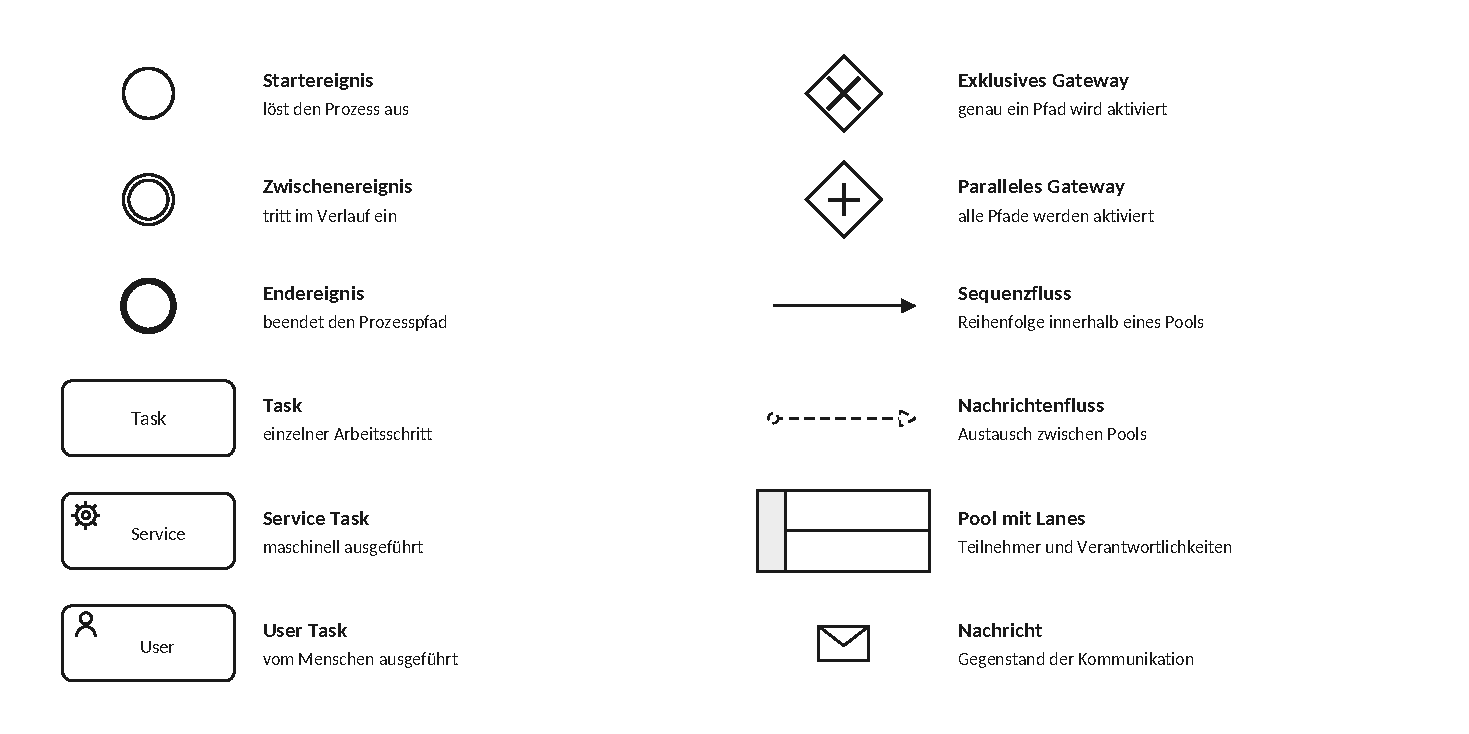
\includegraphics[width=\textwidth]{abb/abb4-bpmn-elemente.pdf}
	\caption{Zentrale BPMN-Notationselemente}
	\label{fig:bpmnelemente}
	\par\vspace{0.4em}{\footnotesize Quelle: In Anlehnung an OMG (2013), S.~25--27.}
\end{figure}

Verst\"andlichkeit entsteht nicht allein aus der Notation. Dumas et al.~empfehlen f\"ur Aktivit\"aten eine Beschriftung aus einem Verb im Imperativ und einem nachfolgenden Substantiv, das ein Gesch\"aftsobjekt bezeichnet, damit Modelle auch ohne vertiefte Vorkenntnisse lesbar bleiben\footcite[Vgl.][S.~75]{Dumas2018}. Zur Muehlen und Recker weisen anhand einer Auswertung realer Modelle nach, dass regelm\"a{\ss}ig weniger als ein F\"unftel des Sprachumfangs tats\"achlich verwendet werde und sich die genutzten Elemente in wiederkehrenden Gruppen b\"undelten\footcite[Vgl.][hier S.~465]{ZurMuehlenRecker2008}; Recker sieht im Umfang des Standards zudem eine Ursache f\"ur Lernaufwand und uneinheitliche Anwendung\footcite[Vgl.][hier S.~188]{Recker2010}. Die Modelle der vorliegenden Arbeit beschr\"anken sich daher auf das beschriebene Kernset, was zugleich den Vergleich von Ist- und Soll-Modell erleichtert. Welche Bedeutung der Notation \"uber die Darstellung hinaus zukommt, behandelt der folgende Abschnitt.

\subsubsection{Relevanz f\"ur die prozessorientierte Digitalisierung}
\label{bpmnDigitalisierung}

BPMN ist in das Business Process Management eingebettet, das Prozesse als organisatorisches Gestaltungsobjekt behandelt. Dumas et al.~gliedern dessen Vorgehen in einen Lebenszyklus, der von der Prozessidentifikation \"uber die Modellierung und Analyse des Ist-Zustandes zum Redesign, zur Implementierung und zum Monitoring f\"uhrt\footcite[Vgl.][S.~22]{Dumas2018}. Die vorliegende Arbeit durchl\"auft diesen Zyklus bis zum Redesign; Implementierung und Monitoring bleiben au{\ss}erhalb des Untersuchungsrahmens.

Weske beschreibt Prozessmodelle als Bindeglied zwischen fachlicher Beschreibung und technischer Umsetzung, da hinreichend pr\"azise Modelle von einer Process Engine ausgef\"uhrt werden k\"onnen\footcite[Vgl.][S.~120]{Weske2024}. F\"ur die Soll-Konzeption ist zudem n\"utzlich, dass ein BPMN-Modell jeden Schritt einem Tr\"ager und jede Verzweigung einer Bedingung zuordnet. Automatisierungsentscheidungen treten dadurch offen zutage, weil das Modell zeigt, welche Schritte maschinell ablaufen und an welchen Stellen ein Mensch entscheidet. Kapitel~3 wendet die Grundlagen dieses Kapitels auf den bestehenden Prozess an und untersucht ihn hinsichtlich seiner Schwachstellen.

